\documentclass{ximera}

 

\usepackage{epsfig}

\graphicspath{
  {./}
  {figures/}
}

\usepackage{morewrites}
\makeatletter
\newcommand\subfile[1]{%
\renewcommand{\input}[1]{}%
\begingroup\skip@preamble\otherinput{#1}\endgroup\par\vspace{\topsep}
\let\input\otherinput}
\makeatother

\newcommand{\includeexercises}{\directlua{dofile("/home/jim/linearAlgebra/laode/exercises.lua")}}

%\newcounter{ccounter}
%\setcounter{ccounter}{1}
%\newcommand{\Chapter}[1]{\setcounter{chapter}{\arabic{ccounter}}\chapter{#1}\addtocounter{ccounter}{1}}

%\newcommand{\section}[1]{\section{#1}\setcounter{thm}{0}\setcounter{equation}{0}}

%\renewcommand{\theequation}{\arabic{chapter}.\arabic{section}.\arabic{equation}}
%\renewcommand{\thefigure}{\arabic{chapter}.\arabic{figure}}
%\renewcommand{\thetable}{\arabic{chapter}.\arabic{table}}

%\newcommand{\Sec}[2]{\section{#1}\markright{\arabic{ccounter}.\arabic{section}.#2}\setcounter{equation}{0}\setcounter{thm}{0}\setcounter{figure}{0}}

\newcommand{\Sec}[2]{\section{#1}}

\setcounter{secnumdepth}{2}
%\setcounter{secnumdepth}{1} 

%\newcounter{THM}
%\renewcommand{\theTHM}{\arabic{chapter}.\arabic{section}}

\newcommand{\trademark}{{R\!\!\!\!\!\bigcirc}}
%\newtheorem{exercise}{}

\newcommand{\dfield}{{\sf dfield9}}
\newcommand{\pplane}{{\sf pplane9}}

\newcommand{\EXER}{\section*{Exercises}}%\vspace*{0.2in}\hrule\small\setcounter{exercise}{0}}
\newcommand{\CEXER}{}%\vspace{0.08in}\begin{center}Computer Exercises\end{center}}
\newcommand{\TEXER}{} %\vspace{0.08in}\begin{center}Hand Exercises\end{center}}
\newcommand{\AEXER}{} %\vspace{0.08in}\begin{center}Hand Exercises\end{center}}

% BADBAD: \newcommand{\Bbb}{\bf}

\newcommand{\R}{\mbox{$\Bbb{R}$}}
\newcommand{\C}{\mbox{$\Bbb{C}$}}
\newcommand{\Z}{\mbox{$\Bbb{Z}$}}
\newcommand{\N}{\mbox{$\Bbb{N}$}}
\newcommand{\D}{\mbox{{\bf D}}}
\usepackage{amssymb}
%\newcommand{\qed}{\hfill\mbox{\raggedright$\square$} \vspace{1ex}}
%\newcommand{\proof}{\noindent {\bf Proof:} \hspace{0.1in}}

\newcommand{\setmin}{\;\mbox{--}\;}
\newcommand{\Matlab}{{M\small{AT\-LAB}} }
\newcommand{\Matlabp}{{M\small{AT\-LAB}}}
\newcommand{\computer}{\Matlab Instructions}
\newcommand{\half}{\mbox{$\frac{1}{2}$}}
\newcommand{\compose}{\raisebox{.15ex}{\mbox{{\scriptsize$\circ$}}}}
\newcommand{\AND}{\quad\mbox{and}\quad}
\newcommand{\vect}[2]{\left(\begin{array}{c} #1_1 \\ \vdots \\
 #1_{#2}\end{array}\right)}
\newcommand{\mattwo}[4]{\left(\begin{array}{rr} #1 & #2\\ #3
&#4\end{array}\right)}
\newcommand{\mattwoc}[4]{\left(\begin{array}{cc} #1 & #2\\ #3
&#4\end{array}\right)}
\newcommand{\vectwo}[2]{\left(\begin{array}{r} #1 \\ #2\end{array}\right)}
\newcommand{\vectwoc}[2]{\left(\begin{array}{c} #1 \\ #2\end{array}\right)}

\newcommand{\ignore}[1]{}


\newcommand{\inv}{^{-1}}
\newcommand{\CC}{{\cal C}}
\newcommand{\CCone}{\CC^1}
\newcommand{\Span}{{\rm span}}
\newcommand{\rank}{{\rm rank}}
\newcommand{\trace}{{\rm tr}}
\newcommand{\RE}{{\rm Re}}
\newcommand{\IM}{{\rm Im}}
\newcommand{\nulls}{{\rm null\;space}}

\newcommand{\dps}{\displaystyle}
\newcommand{\arraystart}{\renewcommand{\arraystretch}{1.8}}
\newcommand{\arrayfinish}{\renewcommand{\arraystretch}{1.2}}
\newcommand{\Start}[1]{\vspace{0.08in}\noindent {\bf Section~\ref{#1}}}
\newcommand{\exer}[1]{\noindent {\bf \ref{#1}}}
\newcommand{\ans}{}
\newcommand{\matthree}[9]{\left(\begin{array}{rrr} #1 & #2 & #3 \\ #4 & #5 & #6
\\ #7 & #8 & #9\end{array}\right)}
\newcommand{\cvectwo}[2]{\left(\begin{array}{c} #1 \\ #2\end{array}\right)}
\newcommand{\cmatthree}[9]{\left(\begin{array}{ccc} #1 & #2 & #3 \\ #4 & #5 &
#6 \\ #7 & #8 & #9\end{array}\right)}
\newcommand{\vecthree}[3]{\left(\begin{array}{r} #1 \\ #2 \\
#3\end{array}\right)}
\newcommand{\cvecthree}[3]{\left(\begin{array}{c} #1 \\ #2 \\
#3\end{array}\right)}
\newcommand{\cmattwo}[4]{\left(\begin{array}{cc} #1 & #2\\ #3
&#4\end{array}\right)}

\newcommand{\Matrix}[1]{\ensuremath{\left(\begin{array}{rrrrrrrrrrrrrrrrrr} #1 \end{array}\right)}}

\newcommand{\Matrixc}[1]{\ensuremath{\left(\begin{array}{cccccccccccc} #1 \end{array}\right)}}



\renewcommand{\labelenumi}{\theenumi)}
\newenvironment{enumeratea}%
{\begingroup
 \renewcommand{\theenumi}{\alph{enumi}}
 \renewcommand{\labelenumi}{(\theenumi)}
 \begin{enumerate}}
 {\end{enumerate}\endgroup}



\newcounter{help}
\renewcommand{\thehelp}{\thesection.\arabic{equation}}

%\newenvironment{equation*}%
%{\renewcommand\endequation{\eqno (\theequation)* $$}%
%   \begin{equation}}%
%   {\end{equation}\renewcommand\endequation{\eqno \@eqnnum
%$$\global\@ignoretrue}}

%\input{psfig.tex}

\author{Martin Golubitsky and Michael Dellnitz}

%\newenvironment{matlabEquation}%
%{\renewcommand\endequation{\eqno (\theequation*) $$}%
%   \begin{equation}}%
%   {\end{equation}\renewcommand\endequation{\eqno \@eqnnum
% $$\global\@ignoretrue}}

\newcommand{\soln}{\textbf{Solution:} }
\newcommand{\exercap}[1]{\centerline{Figure~\ref{#1}}}
\newcommand{\exercaptwo}[1]{\centerline{Figure~\ref{#1}a\hspace{2.1in}
Figure~\ref{#1}b}}
\newcommand{\exercapthree}[1]{\centerline{Figure~\ref{#1}a\hspace{1.2in}
Figure~\ref{#1}b\hspace{1.2in}Figure~\ref{#1}c}}
\newcommand{\para}{\hspace{0.4in}}

\renewenvironment{solution}{\suppress}{\endsuppress}

\ifxake
\newenvironment{matlabEquation}{\begin{equation}}{\end{equation}}
\else
\newenvironment{matlabEquation}%
{\let\oldtheequation\theequation\renewcommand{\theequation}{\oldtheequation*}\begin{equation}}%
  {\end{equation}\let\theequation\oldtheequation}
\fi

\makeatother


\title{mo3.tex}

\begin{document}
\begin{abstract}
BADBAD
\end{abstract}
\maketitle

\chapter{Matrices and Linearity}

\subsection*{Section~\protect{\ref{S:4.1}} Matrix Multiplication of Vectors}
\rhead{S:4.1}{MATRIX MULTIPLICATION OF VECTORS}

\exer{c4.1.1}
\[
Ax =
\left(\begin{array}{rr} 2 & 1 \\ -1 & 4\end{array}\right)
\left(\begin{array}{r} 3 \\ -2\end{array}\right) =
\left(\begin{array}{r} 6 - 2 \\ -3 - 8\end{array}\right) =
\left(\begin{array}{r} 4 \\ -11\end{array}\right)
\]

\exer{c4.1.a3a} $Ax = \vectwo{6}{-10}$.

\exer{c4.1.a3c} $Ax = \left(13\right)$.

\exer{c4.1.b3}
Compute $Ax$ directly:
\[ Ax = \left(\begin{array}{c} x_1a_{11} + x_2a_{12} + \cdots +
x_na_{1n} \\  x_1a_{21} + x_2a_{22} + \cdots + x_na_{2n} \\
\\ \vdots \\ x_1a_{m1} + x_2a_{m2} + \cdots + x_na_{mn}
\end{array}\right) = x_1\left(\begin{array}{r} a_{11} \\ a_{21} \\
\vdots \\ a_{m1} \end{array}\right) + x_2\left(\begin{array}{r}
a_{12} \\ a_{22} \\ \vdots \\ a_{m2} \end{array}\right) + \cdots
+ x_n\left(\begin{array}{r} a_{1n} \\ a_{2n} \\
\vdots \\ a_{mn} \end{array}\right). \]
So, it is indeed true that $Ax = x_1A_1 + x_2A_2 + \cdots
+ x_nA_n$.

\exer{c4.1.4}
\[
\left(\begin{array}{rrr} 2 & 3 & -2 \\ 6 & 0 & -5\end{array}\right) 
\left(\begin{array}{r} x_1 \\ x_2 \\ x_3\end{array}\right) = 
\left(\begin{array}{r} 4 \\ 1\end{array}\right)
\]

\exer{c4.1.7} 
\ans The equations are valid when
\[ A = \left(\begin{array}{rr} 3 & 1 \\ -5 & 4\end{array}\right). \]
\soln Let
\[ A = \left(\begin{array}{rr} a_{11} & a_{12} \\ a_{21} & 
a_{22}\end{array}\right). \]
So
\[ \left(\begin{array}{rr} a_{11} & a_{12} \\ a_{21} & a_{22}\end{array}\right)
\left(\begin{array}{r} 1 \\ 0\end{array}\right) =
\left(\begin{array}{r} 3 \\ -5\end{array}\right) \AND
\left(\begin{array}{rr} a_{11} & a_{12} \\ a_{21} & a_{22}\end{array}\right)
\left(\begin{array}{r} 0 \\ 1\end{array}\right) =
\left(\begin{array}{r} 1 \\ 4.\end{array}\right) \]
These matrix equations are equivalent to the linear equations
\[ \begin{array}{rcl}
a_{11} & = & 3 \\
a_{21} & = & -5 \\
a_{12} & = & 1 \\
a_{22} & = & 4.\end{array} \]

\exer{c4.1.9}
\ans There is no $2 \times 2$ upper triangular matrix $A$ that
satisfies equation \Ref{eq:avect}, but any symmetric matrix $A$ of the form
\[ A = \mattwo{1}{2}{2}{a_{22}}, \]
where $a_{22}$ is a real number, satisfies \Ref{eq:avect}.

\soln Let $A$ be the upper triangular matrix
\[ \mattwo{a_{11}}{a_{12}}{0}{a_{22}}. \]
The resulting matrix equation
\[ \mattwo{a_{11}}{a_{12}}{0}{a_{22}}
\vectwo{1}{0} = \vectwo{1}{2} \]
yields the linear equations
\[ \begin{array}{rcl}
a_{11} & = & 1 \\
0 & = & 2.\end{array} \]
The second equation is inconsistent, so there is no solution.

\para Then let $A$ be the symmetric matrix
\[ \mattwo{a_{11}}{a_{12}}{a_{12}}{a_{22}}. \]
Write the matrix equation
\[ \mattwo{a_{11}}{a_{12}}{a_{12}}{a_{22}}
\vectwo{1}{0} = \vectwo{1}{2}, \]
from which we obtain the consistent linear system
\[ \begin{array}{rcl}
a_{11} & = & 1 \\
a_{12} & = & 2.\end{array} \]

\exer{c4.1.a10b} Load the system into \Matlabp, then type {\tt b = A*x}
to obtain:
\begin{verbatim}
b =
  103.5000
  175.8000
 -296.9000
 -450.1000
  197.4000
  656.6000
  412.4000
\end{verbatim}

\exer{c4.1.11} Using \Matlabp:
\begin{verbatim}
A\b =
   -2.3828
   -1.0682
    0.1794
\end{verbatim}



\subsection*{Section~\protect{\ref{s:4.2}} Matrix Mappings}
\rhead{s:4.2}{MATRIX MAPPINGS}

\exer{c4.2.a1a}
\ans If $x = (x_1,0)^t$, where $x_1$ is any real scalar, then $Ax = 0$.

\soln Let $x = (x_1,x_2)^t$ and solve the system
\[
Ax = \mattwo{0}{1}{0}{-2}\vectwo{x_1}{x_2} = \vectwo{0}{0}
\]
by row reducing $A$ to obtain
\[
\mattwo{0}{1}{0}{0}.
\]
Thus, $Ax = 0$ when $x_2 = 0$.

\exer{c4.2.a1c}
\ans If $x = (x_1,3x_1)^t$, where $x_1$ is any real scalar, then $Cx = 0$.

\soln Solve $Cx = 0$ by row reducing $C$ to find that $Cx = 0$ when
$x_1 - \frac{1}{3}x_2 = 0$.

\exer{c4.2.1b} \ans
\[
R_{(-45^\circ)} = \mattwo{\cos (-45^\circ)}{-\sin
(-45^\circ)}{\sin (-45^\circ)}{\cos (-45^\circ)} =
\mattwo{\frac{1}{\sqrt{2}}}{\frac{1}{\sqrt{2}}}{-\frac{1}{\sqrt{2}}}
{\frac{1}{\sqrt{2}}}.
\]

\exer{c4.2.2a} The map $L_A$ that reflects vectors across the $x$-axis is
$(x,y) \rightarrow (x,-y)$.  The matrix is
\[
A = \mattwo{1}{0}{0}{-1}.
\]

\exer{c4.2.2c} The map $L_A$ that reflects vectors across the line $y=x$ is
$(x,y) \rightarrow (y,x)$.  The matrix is
\[
A = \mattwo{0}{1}{1}{0}.
\]

\exer{c7.8.2}
\ans The matrix
\[ R_{90^\circ} = \mattwo{\cos{90^\circ}}{-\sin{90^\circ}}
{\sin{90^\circ}}{\cos{90^\circ}} = \mattwo{0}{-1}{1}{0} \]
performs the desired transformation.

\soln Note that the transformations $(3,4) \rightarrow (-4,3)$ and
$(1,-2) \rightarrow (2,1)$ are obtained by rotating the plane
$90^\circ$ counterclockwise.  Then use \Ref{e:rotmat} to obtain the
matrix corresponding to this rotation.

\exer{c4.2.3a} The matrix which is a rotation of the plane 
through angle $\theta$ followed by a dilatation $cI_2$ is
\[
cR_\theta =
\mattwo{c\cos\theta}{-c\sin\theta}{c\sin\theta}{c\cos\theta}.
\]
In order for the given matrix to equal $cR_\theta$, we need
\[
\mattwo{a}{-b}{b}{a} =
\mattwo{c\cos\theta}{-c\sin\theta}{c\sin\theta}{c\cos\theta}.
\]
Thus, we have $a = c\cos\theta$ and $b = c\sin\theta$.  We can then write
\[
c^2 = c^2(cos^2\theta + \sin^2\theta) = c^2\cos^2\theta + c^2\sin^2\theta
= a^2 + b^2,
\]
or
\[
c = \sqrt{a^2 + b^2}.
\]

\exer{c4.2.a4a} The matrix $A$ maps any vector $x$ of the form
$x = s(1,1)^t$, where $s$ is a real scalar, to twice its length, and any
vector of the form $x = s(0,1)^t$ to half its length.

\para If you are having trouble finding this vector with {\tt map},
turn on the rescale vectors option, which scales every vector to length
$1$ after mapping it.  Then, test vectors by applying {\sf map} several
times until you find a vector which (approximately) maps to itself.

\newpage
\exer{c4.2.a4c} The matrix $C$ maps any vector of the form $x = s(1,0)$
to twice its length and maps any vector of the form $x = s(1,2)$ to
$-\frac{1}{2}$ times its length.

\exer{c4.2.bb} \ans Matrix $B$ rotates the plane by $\theta =
\approx 3.0585$ counterclockwise and dilatates it by a factor of
$c = \sqrt{5.8} \approx 2.4083$.

\soln Matrix $B$ is a special case of Exercise~\ref{c4.2.3a} with $a = -2.4$
and $b = 0.2$.  Thus, $c = \sqrt{a^2 + b^2} = \sqrt{5.8}$ and
$\theta = \cos^{-1}\left(\frac{a}{\sqrt{a^2 + b^2}}\right) =
\cos^{-1}\left(-\frac{2.4}{\sqrt{(-2.4)^2 + (0.2)^2}}\right) \approx 3.0585$.

\exer{c4.2.4a} $A$ rotates the plane $30^\circ$ clockwise.

\exer{c4.2.4c} $C$ reflects the plane across the line $y = x$.

\exer{c4.2.4e} $E$ maps $(x,y)$ to a point on the line $y = x$; that
point is $(\frac{x + y}{2}, \frac{x + y}{2})$.



\subsection*{Section~\protect{\ref{S:linearity}} Linearity}
\rhead{S:linearity}{LINEARITY}

\exer{c4.3.1}
(a) $2(2,4) - 3(3,-1) = (-5,11)$;

(b) $10(1,0,-1) - 2(2,-4,3) = (6,8,-16)$;

(c) $5(4,2,-1,1) - 1(-1,3,5,7) = (21,7,-10,-2)$.

\exer{c4.3.3}
The equation
\[ (-2, -1) = \alpha(1,2) + \beta(1,-3) =
(\alpha + \beta, 2\alpha - 3\beta ) \]
can be rewritten as the linear system
\[ \begin{array}{rrrrr}
-2 & = & \alpha & + & \beta \\
-1 & = & 2\alpha & - & 3\beta\end{array}. \]
Solving this system yields $\alpha = -\frac{7}{5}$ and
$\beta = -\frac{3}{5}$.

\exer{c4.3.5}
\ans The equation
\[ \alpha(3,-2) + \beta(2,3) + \gamma(1,4) = (1,-2) \]
holds for any real numbers $\alpha$,$\beta$,
$\gamma$ such that $\alpha = \frac{5}{13}\gamma +
\frac{7}{13}$ and $\beta = -\frac{14}{13}\gamma
- \frac{4}{13}$.

\soln Write the equation as the linear system
\[ \begin{array}{rrrrrrl}
3\alpha & + & 2\beta & + & \gamma & = & 1 \\
-2\alpha & + & 3\beta & + & 4\gamma & = & -2. \end{array} \]
The augmented matrix
\[ \left(\begin{array}{rrr|r}
3 & 2 & 1 & 1 \\
-2 & 3 & 4 & -2 \end{array}\right) \]
row reduces to
\[ \left(\begin{array}{rrr|r}
1 & 0 & -\frac{5}{13} & \frac{7}{13} \\
0 & 1 & \frac{14}{13} & -\frac{4}{13} \end{array}\right) \]
and the equation is valid for any values of $\alpha$,$\beta$,
and $\gamma$ that satisfy this system.

\exer{c4.3.6b} \ans The transformation $T(x,y) = (x + xy, 2y)$ is not linear.

\soln If $T$ is a linear transformation, then
\[
T(x_1 + x_2,y_1 + y_2) = T(x_1,y_1) + T(x_2,y_2)
\]
for any real numbers $x_1$,$x_2$,$y_1$,$y_2$.  However,
\[
\begin{array}{rcl}
T(1,1) & = & (2,2) \\
T(1,0) + T(0,1) & = & (1,0) + (0,2) = (1,2).\end{array}
\]
Therefore $T(1,1) \neq T(1,0) + T(0,1)$ and $T$ is not linear.

\exer{c4.3.6d} The transformation $T(x,y) = (1,x + y, 2y)$ is not linear
because $T(0,0) = (1,0,0) \neq 0$.

\exer{c4.3.8}
\ans The matrix of linear mapping $L$ is
\[
A = \matthree{0}{-1}{-1}{1}{0}{2}{1}{-2}{0}.
\]

\soln Let $X = (x_1,x_2,x_3)$ and let $Y = (y_1,y_2,y_3)$.  
Since $K = (2,1,-1)$,
\[
L(X) = (x_1,x_2,x_3) \times K = 
(-x_2 - x_3, x_1 + 2x_3, x_1 - 2x_2).
\]

To show that $L(X)$ is a linear mapping, first demonstrate that
\Ref{sum} is valid:
\[
\begin{array}{rcl}
L(X + Y) & = & L(x_1 + y_1,x_2 + y_2,x_3 + y_3) \\
& = & (-(x_2 + y_2) - (x_3 + y_3), (x_1 + y_1) + 2(x_3 + y_3),
(x_1 + y_1) - 2(x_2 + y_2)) \\
& = & (-x_2 - x_3, x_1 + 2x_3, x_1 - 2x_2) +
(-y_2 - y_3, y_1 + 2y_3, y_1 - 2y_2) \\
& = & L(X) + L(Y), \end{array}
\]
then show that \Ref{product} is valid:
\[
\begin{array}{rcl}
cL(X) & = & cL(x_1,x_2,x_3) \\
& = & c(-x_2 - x_3, x_1 + 2x_3, x_1 - 2x_2) \\
& = & (-cx_2 - cx_3, cx_1 + 2cx_3, cx_1 - 2cx_2) \\
& = & L(cx_1,cx_2,cx_3) \\
& = & L(cX). \end{array}
\]

Find $A$ by noting that $L(e_j) = Ae_j$ is the $j^{th}$ column of $A$,
and computing
\[ \begin{array}{l}
L(e_1) = L(1,0,0) = (0,1,1) \\
L(e_2) = L(0,1,0) = (-1,0,-2) \\
L(e_3) = L(0,0,1) = (-1,2,0). \end{array} \]

\exer{c4.3.10}
\ans The matrix of linear mapping $L_A$ is
\[ A = \matthree{0}{1}{0}{0}{0}{1}{1}{0}{0}. \]

\soln Note that if $\sigma = L_A$, then $\sigma(e_j) = Ae_j$ is the
$j^{th}$ column of matrix $A$.  Thus $A$ is determined by
\[
\begin{array}{l}
\sigma(e_1) = \sigma(1,0,0) = (0,0,1) \\
\sigma(e_2) = \sigma(0,1,0) = (1,0,0) \\
\sigma(e_3) = \sigma(0,0,1) = (0,1,0). \end{array}
\]

\exer{c4.3.12}
The mapping $L(x)$ is linear if $L(x + y) = L(x) + L(y)$ and
if $cL(x) = L(cx)$.  We can use the assumption that $L_1(x)$
and $L_2(x)$ are linear mappings to show:
\[ \begin{array}{rcl}
L(x + y) & = & L_1(x + y) + L_2(x + y) \\
& = & L_1(x) + L_1(y) + L_2(x) + L_2(y) \\
& = & [L_1(x) + L_2(x)] + [L_1(y) + L_2(y)] \\
& = & L(x) + L(y) \end{array} \]
and
\[ \begin{array}{rcl}
cL(x) & = & cL_1(x) + cL_2(x) \\
& = & L_1(cx) + L_2(cx) \\
& = & L(cx). \end{array} \]

Assume that $L = L_A$, $L_1 = L_{A_1}$ and $L_2 = L_{A_2}$ for
$m \times n$ matrices $A$, $A_1$, $A_2$.  We claim that
$A = A_1 + A_2$, where $A_1 + A_2$ is the matrix obtained by
adding corresponding entries of $A_1$ and $A_2$.  By
definition, $L(e_j) = L_1(e_j) + L_2(e_j)$.  Lemma~\ref{columnsA}
implies that the $j^{th}$ column of $A$ is the sum of the
$j^{th}$ columns of $A_1$ and $A_2$ for all columns {j}, so
$A = A_1 + A_2$.

\exer{c4.3.14}
The mapping $L_A$ performs the transformation $(x,y) \rightarrow
(0.5y, -0.5x)$.  That is, the mapping rotates a 2-vector
$90^\circ$ clockwise then halves its length.

\exer{c4.3.15B} Typing either {\tt A*(x + y)} or {\tt A*x + A*y} yields
\begin{verbatim}
ans =
   -19
   -15
    24
     3
    15
\end{verbatim}
verifying \Ref{sum}.  Typing {\tt c*(A*x)} or {\tt A*(c*x)} yields
\begin{verbatim}
ans =
  -156
  -364
  -455
  -273
  -117
\end{verbatim}
verifying \Ref{product}.



\subsection*{Section~\protect{\ref{S:Superposition}} The Principle of
Superposition}
\rhead{S:Superposition}{THE PRINCIPLE OF SUPERPOSITION}

\exer{c4.4.1}
(a) \ans All solutions can be written as a superposition of the vectors
\[
v_1 = \vecthree{-1}{1}{0} \AND v_2 = \vecthree{-1}{0}{1}.
\]

\soln The equation $x + y + z = 0$ is a linear system of three variables
in one equation.  If we consider $y$ and $z$ to be free variables, then
every solution to the system has the form
\[
\vecthree{x}{y}{z} = \left(\begin{array}{c} -y - z \\ y \\
z \end{array}\right) = y\vecthree{-1}{1}{0} +
z\vecthree{-1}{0}{1}.
\]

(b) \ans All solutions can be written as a superposition
of the second pair of vectors
\[
w_1 = \vecthree{1}{0}{-1} \AND w_2 = \vecthree{0}{1}{-1}.
\]

\soln Write the same linear system, but this time consider $x$ and $y$
to be free variables.  In this case, every solution has the form:
\[
\vecthree{x}{y}{z} = \left(\begin{array}{c} x \\ y \\
-x - y \end{array}\right) = x\vecthree{1}{0}{-1} +
z\vecthree{0}{1}{-1}.
\]

\exer{c4.4.3}
(a) \ans All solutions to the homogeneous equation are of the form
\[
x = \vecthree{x_1}{x_2}{x_3} = s\vecthree{-11}{7}{1}.
\]

\soln Row reduce the matrix of the homogeneous system
$Ax = 0$ to obtain:
\[
\left(\begin{array}{rrr} 1 & 0 & 11 \\ 0 & 1 & -7 \end{array}\right).
\]
So $x_1 = -11s$, $x_2 = 7s$ and $x_3 = s$.

(b) \ans One possible solution is
\[ \vecthree{x_1}{x_2}{x_3} = \vecthree{1}{1}{1}. \]

\soln Assign a value to $x_3$, then substitute into the two equations
of the inhomogeneous system to obtain values for $x_1$ and $x_2$.

(c) All solutions to \Ref{E:inhom} can be found by adding a
single solution of the inhomogeneous system to all solutions
of the homogeneous system, so:
\[
x = \vecthree{1}{1}{1} + s\vecthree{-11}{7}{1}.
\]



\subsection*{Section~\protect{\ref{S:4.6}} Composition and Multiplication
of Matrices}
\rhead{S:4.6}{COMPOSITION AND MULTIPLICATION OF MATRICES}

\exer{c4.6.-1a} $AB=\mattwo{-2}{0}{7}{-1}$ and $BA= \mattwo{-2}{0}{5}{-1}$.

\exer{c4.6.-1c} $AB$ is not defined.  $BA$ is not defined.  

\exer{c4.6.0a}
$\mattwo{2}{3}{0}{1}\mattwo{-1}{1}{-3}{2} =
\cmattwo{-2 - 9}{2+6}{-3}{2} = \mattwo{-11}{8}{-3}{2}$.

\exer{c4.6.0c} $\left(\begin{array}{rr} 2 & 3\\ -2 & 5 \\1 & -1 \end{array}
\right) \left(\begin{array}{rrr} 1 & 2 & 3\\ -2 & 3 & -1 \end{array}\right)
= \matthree{-4}{13}{3}{-12}{11}{-11}{3}{-1}{4}$.

\exer{c4.6.1}
\ans For any matrix $B$ of the form
\[
\mattwo{b_{11}}{0}{0}{b_{22}}
\]
the equation $AB = BA$ is valid.

\soln Let
\[
B = \mattwo{b_{11}}{b_{12}}{b_{21}}{b_{22}}.
\]
Then compute the matrix $B$ for which
\[
\begin{array}{rcl}
AB & = & BA \\
\mattwo{2}{0}{0}{-1}\mattwo{b_{11}}{b_{12}}{b_{21}}{b_{22}} &
= & \mattwo{b_{11}}{b_{12}}{b_{21}}{b_{22}}\mattwo{2}{0}{0}{-1} \\
\mattwo{2b_{11}}{2b_{12}}{-b_{21}}{-b_{22}} & = &
\mattwo{2b_{11}}{-b_{12}}{2b_{21}}{-b_{22}} \end{array}
\]
which is equivalent to the linear system
\[
\begin{array}{l}
2b_{11} = 2b_{11} \\
2b_{12} = -b_{12} \\
-b_{21} = 2b_{21} \\
-b_{22} = -b_{22}. \end{array}
\]

\exer{c4.6.3}
\[ AA^t = \matthree{1}{0}{-3}{-2}{1}{1}{0}{1}{-5}
\matthree{1}{-2}{0}{0}{1}{1}{-3}{1}{-5} =
\matthree{10}{-5}{15}{-5}{6}{-4}{15}{-4}{26}. \]

\exer{c4.7.1b} The matrix $AB$ is not defined because $A$ has 5 columns
while $B$ has four rows.  The matrix $BA$ is also not defined
because $B$ has 6 columns and $A$ has 3 rows.



\subsection*{Section~\protect{\ref{S:4.7}} Properties of Matrix Multiplication}
\rhead{S:4.7}{PROPERTIES OF MATRIX MULTIPLICATION}

\exer{c4.7.2.2}  Let $B = AA^t$, where $A$ is an $m \times n$ matrix.
Then $B^t = (AA^t)^t = (A^t)^tA^t$ by \Ref{e:transposeprod}.  Since
$(A^t)^t=A$, $B^t=AA^t=B$ and $B$ is symmetric.  Similarly, $C = A^tA$
is symmetric.

\exer{c4.7.4}
\[ 
B = I + A + \frac{1}{2}A^2 =
 \matthree{1}{0}{0}{0}{1}{0}{0}{0}{1} +
\matthree{0}{1}{0}{0}{0}{1}{0}{0}{0} +
\matthree{0}{0}{\frac{1}{2}}{0}{0}{0}{0}{0}{0}
= \matthree{1}{1}{\frac{1}{2}}{0}{1}{1}{0}{0}{1}. \]
\[ 
C = I + tA + \frac{1}{2}(tA)^2 
= \matthree{1}{0}{0}{0}{1}{0}{0}{0}{1} +
\matthree{0}{t}{0}{0}{0}{t}{0}{0}{0} +
\cmatthree{0}{0}{\frac{t^2}{2}}{0}{0}{0}{0}{0}{0}
= \cmatthree{1}{t}{\frac{t^2}{2}}{0}{1}{t}{0}{0}{1}. \]

\exer{c4.7.8}
Let $A$ and $B$ be $n \times n$ upper triangular matrices.  To show
that $AB$ is upper triangular, we must show that if $i > j$, then
\[ (ab)_{ij} = \sum_{k = 1}^{n} a_{ik}b_{kj} = 0. \]
For every component of this sum, either $i > k$, in which case $a_{ik}
= 0$ since $A$ is upper-triangular, or $i \leq k$, in which case, since
$i > j$, $k > j$, so $b_{kj} = 0$.  Therefore, for all $i > j$,
$(ab)_{ij} = 0$, so $AB$ is upper triangular.

\exer{c4.7.0b} Computer experiment.

\exer{c4.7.2} Computer experiment.



\subsection*{Section~\protect{\ref{S:SLS}} Solving Linear Systems and Inverses}
\rhead{S:SLS}{SOLVING LINEAR SYSTEMS AND INVERSES}

\exer{c4.8.1}
If two matrices are inverses of each other, then their product is the
identity matrix.  So:
\[ \matthree{1}{0}{2}{0}{-1}{2}{1}{0}{1}
\matthree{-1}{0}{2}{2}{-1}{-2}{1}{0}{-1} =
\matthree{1}{0}{0}{0}{1}{0}{0}{0}{1}. \]

\exer{c4.8.3}
\ans The matrix $A$ is invertible for $a \neq 0$ and $b \neq 0$.

\soln By Theorem~\ref{invertequiv}, a matrix is invertible if it is row
equivalent to the identity matrix.  If $a = 0$ or if $b = 0$, then
$A$ is not row equivalent to $I_2$ and is therefore not invertible.

\exer{c4.9.3a} \ans
$A^{-1} = \dps\frac{1}{10}\matthree{-8}{32}{-9}{2}{2}{1}{2}
{-8}{1}$.

\soln Let
\[
M = (A|I_3) = \left(\begin{array}{rrr|rrr} 1 & 4 & 5 & 1 & 0 & 0 \\
0 & 1 & -1 & 0 & 1 & 0 \\
-2 & 0 & -8 & 0 & 0 & 1 \end{array}\right).
\]
Then, row reduce $M$ to obtain the augmented matrix $(I_3|A^{-1})$.

\exer{c4.8.5}
The matrix $A$ is invertible with inverse $B = -(A^2 + a_2A + a_1)$.
To show this, note that
\[ AB = A(-(A^2 + a_2A + a_1)) = I_n \]
if and only if $A^3 + a_2A^2 + a_1A = -I_n$.  This condition is valid
by definition of $A$, so $A$ is invertible.

\newpage
\exer{c4.9.6}
\ans
The matrix $A$ is invertible for any choice of $a$, $b$, and $c$, and
\[
A^{-1} = \left(\begin{array}{rrc} 1 & -a & -b + ac \\ 0 & 1 & -c 
\\ 0 & 0 & 1 \end{array}\right).
\]

\soln Theorem~\ref{invertequiv} states that a matrix is invertible if
it is row equivalent to $I_n$.  By row reducing the augmented matrix
$(A|I_3)$ as follows:
\[
\left(\begin{array}{rrr|rrr} 1 & a & b & 1 & 0 & 0 \\
0 & 1 & c & 0 & 1 & 0 \\ 0 & 0 & 1 & 0 & 0 & 1
\end{array}\right) \rightarrow \left(\begin{array}{rrr|rrc}
1 & 0 & 0 & 1 & -a & -b + ac \\ 0 & 1 & 0 & 0 & 1 & -c \\
0 & 0 & 1 & 0 & 0 & 1 \end{array}\right)
\]
we show that $A$ is invertible for any choice of $a$, $b$, and
$c$, and find a value for $A^{-1}$.

\exer{c4.9.7b}
Type {\tt N = [B eye(4)]} in \Matlabp, then row reduce {\tt N} to obtain:
\begin{verbatim}
ans =
1.0000        0        0        0   -1.5714   -0.4286         0    1.4286
     0   1.0000        0        0    0.7429    0.0571    0.2000   -0.4571
     0        0   1.0000        0   -0.9143    0.3143   -0.4000    0.4857
     0        0        0   1.0000   -0.6000   -0.2000   -0.2000    0.6000
\end{verbatim}
The command {\tt inv(B)} returns the right half of this augmented
matrix:
\begin{verbatim}
ans =
   -1.5714   -0.4286         0    1.4286
    0.7429    0.0571    0.2000   -0.4571
   -0.9143    0.3143   -0.4000    0.4857
   -0.6000   -0.2000   -0.2000    0.6000
\end{verbatim}



\subsection*{Section~\protect{\ref{S:det2x2}} Determinants of $2\times 2$ Matrices}
\rhead{S:det2x2}{DETERMINANTS OF $2\times 2$ MATRICES}

\exer{c4.9.1}
Use \Ref{e:formAinv} to compute the inverse of the matrix,
as follows:
\[ \mattwo{2}{1}{3}{2}^{-1} = \frac{1}{4-3}\mattwo{2}{-1}{-3}{2}
= \mattwo{2}{-1}{-3}{2}. \]

\exer{c4.9.4}
Case: $a \neq 0$.  $A$ can be row reduced as follows:
\[ \mattwo{a}{b}{c}{d} \rightarrow
\mattwo{1}{\frac{b}{a}}{c}{d} \rightarrow
\cmattwo{1}{\frac{b}{a}}{0}{\frac{ad - bc}{a}}. \]
If $ad - bc \neq 0$, then the matrix can be row reduced to $I_2$, whereas
if $ad - bc = 0$, the row reduced matrix is:
\[ \mattwo{1}{\frac{b}{a}}{0}{0} \]
which cannot be reduced further and is not row equivalent to $I_2$.

Case: $a = 0$.  If either $c = 0$ or $b = 0$, then the resulting matrices,
\[ \mattwo{0}{b}{0}{d} \AND \mattwo{0}{0}{c}{d} \]
respectively, are not row equivalent to $I_2$, and $ad - bc = 0 - 0 = 0$.
If $c \neq 0$ and $b \neq 0$, then the matrix can be row reduced:
\[ \mattwo{0}{b}{c}{d} \rightarrow
\mattwo{c}{d}{0}{b} \rightarrow \mattwo{1}{\frac{d}{c}}{0}{b} \]
which is row equivalent to $I_2$.  So $A$ is indeed row equivalent
to $I_2$ if and only if $ad - bc \neq 0$.

\exer{c6.4.4}
Verify by computation:
\[ \det(A^{-1}) = \frac{a}{\det(A)}\frac{d}{\det(A)} -
\frac{-b}{\det(A)}\frac{-c}{\det(A)} = \frac{ad - bc}{(\det(A))^2} =
\frac{1}{\det(A)}. \]

\exer{c7.8.4A}
The general system of linear equations in two unknowns is:
\begin{eqnarray*}
a_{11}x_1+a_{12}x_2 & = & b_1\\
a_{21}x_1+a_{22}x_2 & = & b_2.
\end{eqnarray*}
Subtract $a_{11}$ times the $2^{nd}$ equation from $a_{21}$ times the $1^{st}$ 
equation to eliminate $x_1$ and obtain
\[
(a_{21}a_{12}-a_{11}a_{22})x_2 = (a_{21}b_1-a_{11}b_2).
\]
Therefore
\[
x_2 =  \frac{a_{21}b_1-a_{11}b_2}{a_{21}a_{12}-a_{11}a_{22}}
= \frac{\det(B_2)}{\det(A)}.
\]
A similar argument works for $x_1$.

\exer{c7.8.4C} \ans  $y=\frac{29}{11}$.

\soln By Cramer's rule (see \Ref{E:cramer}),
\[
y = \det\mattwo{4}{-1}{1}{7}\left/\det\mattwo{4}{-3}{1}{2}=\frac{29}{11}\right..
\]

\newpage
\exer{c3.8.AA} \ans The matrix $A$ is invertible and $\det(A) = 4$.

\soln Figure~\ref{c3.8.AA} shows the {\tt map} output for this matrix.
The area of the square resulting from the map is $4$, so $|\det(A)| = 4$.

\exer{c3.8.AC} \ans The matrix $A$ is not invertible and $\det(A) = 0$.

\soln Figure~\ref{c3.8.AC} shows the {\tt map} output for this matrix.
The square is mapped to a line, whose area is $0$, so $|\det(A)| = 0$.

\begin{figure}[htb]
                       \centerline{%
                       \psfig{file=exfigure/3-8-AA.eps,width=2.75in}
                       \psfig{file=exfigure/3-8-AC.eps,width=2.75in}}
	\centerline{Figure~\ref{c3.8.AA}\hspace{2.1in}Figure~\ref{c3.8.AC}}
\end{figure}
\end{document}
